% \iffalse
\let\negmedspace\undefined
\let\negthickspace\undefined
\documentclass[journal,12pt,twocolumn]{IEEEtran}
\usepackage{cite}
\usepackage{amsmath,amssymb,amsfonts,amsthm}
\usepackage{algorithmic}
\usepackage{graphicx}
\usepackage{textcomp}
\usepackage{xcolor}
\usepackage{txfonts}
\usepackage{listings}
\usepackage{enumitem}
\usepackage{mathtools}
\usepackage{gensymb}
\usepackage{comment}
\usepackage[breaklinks=true]{hyperref}
\usepackage{tkz-euclide} 
\usepackage{listings}
\usepackage{gvv}                                        
\def\inputGnumericTable{}                                 
\usepackage[latin1]{inputenc}                                
\usepackage{color}                                            
\usepackage{array}                                            
\usepackage{longtable}                                       
\usepackage{calc}                                             
\usepackage{multirow}                                         
\usepackage{hhline}                                           
\usepackage{ifthen}                                           
\usepackage{lscape}
\newtheorem{theorem}{Theorem}[section]
\newtheorem{problem}{Problem}
\newtheorem{proposition}{Proposition}[section]
\newtheorem{lemma}{Lemma}[section]
\newtheorem{corollary}[theorem]{Corollary}
\newtheorem{example}{Example}[section]
\newtheorem{definition}[problem]{Definition}
\newcommand{\BEQA}{\begin{eqnarray}}
\newcommand{\EEQA}{\end{eqnarray}}
\newcommand{\define}{\stackrel{\triangle}{=}}
\theoremstyle{remark}
\newtheorem{rem}{Remark}
\begin{document}

\bibliographystyle{IEEEtran}
\vspace{3cm}

\title{10.5.3.9}
\author{EE23BTECH11063 - Vemula Siddhartha
}
\maketitle
\newpage
\bigskip

\renewcommand{\thefigure}{\theenumi}
\renewcommand{\thetable}{\theenumi}
\textbf{Question}:\\
If the sum of first 7 terms of an AP is 49 and that of 17 terms is 289, find the sum of
first n terms.
\\\\
\textbf{Solution: }\\
\begin{align}
S_n=\frac{n}{2}\,\brak{2x\brak{0}+\brak{n-1}\,d}\label{eq10.5.3.9.1}
\end{align}
\begin{align}
S_7&=49 \\
49&=\frac{7}{2}\,\brak{2x\brak{0}+\brak{7-1}\,d}  \\
49&=\frac{7}{2}\,\brak{2x\brak{0}+6d}  \\
x\brak{0}+3d&=7\label{eq10.5.3.9.2}
\end{align}
\begin{align}
S_{17}&=289  \\
289&=\frac{17}{2}\,\brak{2x\brak{0}+\brak{17-1}\,d}  \\
289&=\frac{17}{2}\,\brak{2x\brak{0}+16d}  \\
x\brak{0}+8d&=17 \label{eq10.5.3.9.3}
\end{align}
From  equations \ref{eq10.5.3.9.2} and \ref{eq10.5.3.9.3}, the augmented matrix is:
\begin{align}\vspace{3cm}
 \begin{pmatrix}
1&3&7\\
1&8&17
 \end{pmatrix}
 \\
 R_2\rightarrow R_2-R_1\notag\\
 \begin{pmatrix}
    1&3&7\\
    0&5&10
 \end{pmatrix}
 \\
 R_1\rightarrow 5R_1-3R_2\notag\\
 \begin{pmatrix}
    5&0&5\\
    0&5&10
 \end{pmatrix}
 \\
 R_1\rightarrow\frac{1}{5}R_1\notag\\ R_2\rightarrow\frac{1}{5}R_2\notag\\
 \begin{pmatrix}
    1&0&1\\
    0&1&2
 \end{pmatrix}\\
 \implies
 \begin{pmatrix}
    x\brak{0}\\
    d
 \end{pmatrix}
 =
 \begin{pmatrix}
    1\\2
 \end{pmatrix}
\end{align}
\begin{align}
\implies S_n&= \frac{n}{2}\,\brak{2x\brak{0}+\brak{n-1}\,d}\label{eq10.5.3.9.4}\\
S_n&=n^2\label{eq10.5.3.9.5}
\end{align}
\begin{align}
    x\brak{n}&=\brak{x\brak{0}+nd}u\brak{n}\\
    \implies x\brak{n}&= \brak{1+2n}u\brak{n}\\
    &x\brak{n}\system{Z}X\brak{z}\\
    X\brak{z}&= \sum_{n=-\infty}^{\infty}\brak{1+2n}u\brak{n} z^{-n}\\
    X\brak{z}&=0+\sum_{n=0}^{\infty}\brak{1+2n} z^{-n}\\
    \text{If: }\notag &x\brak{n}\system{Z}X\brak{z}\\
    \implies n^k&x\brak{n}\system{Z}\brak{-1}^{k}z^k\frac{d^k}{dz^k}\brak{X\brak{z}}\notag\\
    \implies X\brak{z}&=\frac{1+z^{-1}}{\brak{1-z^{-1}}^2} \;\;\cbrak{z\in\mathbb{C}: |z|>1}
\end{align}

\begin{figure}[h]
    \centering
    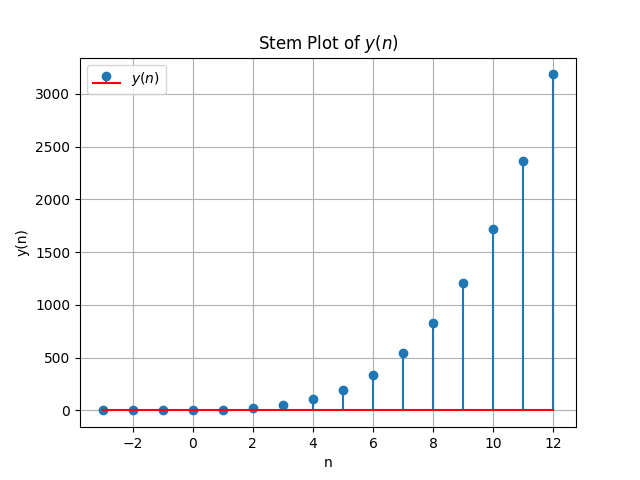
\includegraphics[width=1.1\linewidth]{Figure_1.png}
    \caption{Stem Plot of x(n)}
    \label{stemplot}
\end{figure}
Generalizing the problem:\\
Let the sum of first $n_1$ terms of the AP be 49, and the sum of first $n_2$ terms of the AP be 289.\\
From equation \ref{eq10.5.3.9.1}:
\begin{align}
\implies \frac{n_1}{2}\,\brak{2x\brak{0}+\brak{n_1-1}\,d}&=49\\
\implies n_1x\brak{0}+ d\,\frac{\brak{n_1-1}\brak{n_1}}{2}&=49\label{eq10.5.3.9.10}
\end{align}
Also,
\begin{align}
\frac{n_2}{2}\,\brak{2x\brak{0}+\brak{n_1-1}\,d}&=289\\
\implies x\brak{0}\brak{n_2}+ d\,\frac{\brak{n_2-1}\brak{n_2}}{2}&=289\label{eq10.5.3.9.11}
\end{align}
From  equations \ref{eq10.5.3.9.10} and \ref{eq10.5.3.9.11}, the augmented matrix is:
\begin{align}
    \begin{pmatrix}
        n_1&\frac{\brak{n_1-1}\brak{n_1}}{2}&49\\
        n_2&\frac{\brak{n_2-1}\brak{n_2}}{2}&289
    \end{pmatrix}
    \\R_1\rightarrow\frac{1}{n_1}R_1\notag\\
    \begin{pmatrix}
        1&\frac{\brak{n_1-1}}{2}&\frac{49}{n_1}\\
        n_2&\frac{n_2\,\brak{n_2-1}}{2}&289
    \end{pmatrix}\\
    R_2 \rightarrow R_2-n_2R_1\notag\\
    \begin{pmatrix}
        1&\frac{\brak{n_1-1}}{2}&\frac{49}{n_1}\\
        0&\frac{n_2\,\brak{n_2-n_1}}{2}&289-\frac{49}{n_1}
    \end{pmatrix}\\
    R_2\rightarrow\frac{2}{n_2\brak{n_2-n_1}}R_2\notag\\
    \begin{pmatrix}
        1&\frac{\brak{n_1-1}}{2}&\frac{49}{n_1}\\
        0&1&\frac{2\brak{49n_2-289 n_1}}{n_1 n_2\brak{n_1-n_2}}
    \end{pmatrix}
\end{align}
\begin{align}
    &R_1\rightarrow R_1-\brak{\frac{n_1-1}{2}} R_2\notag\\
    &\begin{pmatrix}
        1 & 0 & \frac{289 n_1^2-289 n_1-49n_2^2+49 n_2}{n_1 n_2\brak{n_1-n_2}} \\\\
        0 & 1 & \frac{2\brak{-289 n_1+49 n_2}}{n_1 n_2\brak{n_1-n_2}}
    \end{pmatrix}\\\notag\\
    \implies &x\brak{0}=49\brak{\frac{-n_2+1}{n_1^2-n_1n_2}}+289\brak{\frac{-n_1+1}{n_2^2-n_1n_2}}\label{eq10.5.3.9.12}\\
    \implies &d=49\brak{\frac{2}{n_1^2-n_1n_2}}+289\brak{\frac{2}{n_2^2-n_1n_2}}\label{eq10.5.3.9.13}
\end{align}
 From the equations \ref{eq10.5.3.9.4}, \ref{eq10.5.3.9.12} and \ref{eq10.5.3.9.13}:
 \begin{align}
     \implies S_n = \frac{n}{2}\,\brak{2\brak{49\brak{\frac{-n_2+1}{n_1^2-n_1n_2}}}+289\brak{\frac{-n_1+1}{n_2^2-n_1n_2}}}\notag\\
     +\brak{n-1}\,\brak{49\brak{\frac{2}{n_1^2-n_1n_2}}+289\brak{\frac{2}{n_2^2-n_1n_2}}}
 \end{align}
 The general term of the AP is:
 \begin{align}
    x\brak{n}= 49\brak{\frac{-n_2+1}{n_1^2-n_1n_2}}+289\brak{\frac{-n_1+1}{n_2^2-n_1n_2}} +\notag\\
    n\brak{49\brak{\frac{2}{n_1^2-n_1n_2}}+289\brak{\frac{2}{n_2^2-n_1n_2}}}\\
    \forall\;\; n\geq0\notag\\
    \implies x\brak{n}= \brak{49\brak{\frac{-n_2+1}{n_1^2-n_1n_2}}+289\brak{\frac{-n_1+1}{n_2^2-n_1n_2}} +\notag\\
    n\brak{49\brak{\frac{2}{n_1^2-n_1n_2}}+289\brak{\frac{2}{n_2^2-n_1n_2}}}}u\brak{n}
 \end{align}
 \begin{table}[h]
    \centering
    \begin{tabular}[12pt]{ |c| c| c|}
    \hline
    \textbf{Variable} & \textbf{Description} &\textbf{Value}\\ 
    \hline
    $x\brak{0}$ & First term of the AP &1\\
    \hline 
    $d$ & Common difference of the AP& 2\\
    \hline
    $S_n$ & Sum of $n$ terms of the AP& $n^2$\\
    \hline
    $S_7$& Sum of 7 terms of the AP& 49\\
    \hline
    $S_{17}$& Sum of 17 terms of the AP&289\\
    \hline
    $x(n)$ & General term& $\brak{1+2n}\,u\brak{n}$\\
    \hline
    $X(z)$ & Z- transform of $x(n)$& $\frac{1+z^{-1}}{\brak{1-z^{-1}}^2} \cbrak{z\in\mathbb{C}: |z|>1}$\\
    \hline    
    \end{tabular}
    \caption{Variables Used}
\end{table}
\end{document}  